\documentclass[12pt]{article}

%%%%%%%%%%%%%%%%%%%%%%%%%%%%%%%%%%%%%%%%%%%%%%%%%%%%%%%%%%%%%%%%%%%%%%%%%%%%%%%%
%                           Package preset for homework
%%%%%%%%%%%%%%%%%%%%%%%%%%%%%%%%%%%%%%%%%%%%%%%%%%%%%%%%%%%%%%%%%%%%%%%%%%%%%%%%
% Miscellaneous
\usepackage[margin=1in]{geometry}
\usepackage[utf8]{inputenc}
\usepackage{indentfirst}
\usepackage{blindtext}
\usepackage{graphicx}
\usepackage{xr-hyper}
\usepackage{hyperref}
\usepackage{enumitem}
\usepackage{color}
\usepackage{float}
% Math
\usepackage{latexsym}
\usepackage{amsfonts}
\usepackage{amssymb}
\usepackage{amsmath}
\usepackage{commath}
\usepackage{amsthm}
\usepackage{bbold}
\usepackage{bm}
% Physics
\usepackage{physics}
\usepackage{siunitx}
% Code typesetting
\usepackage{listings}
% Citation
\usepackage[authoryear]{natbib}
\usepackage{appendix}
\usepackage[capitalize]{cleveref}
% Title & name
\title{Homework}
\author{Tien Vo}
\date{\today}


%%%%%%%%%%%%%%%%%%%%%%%%%%%%%%%%%%%%%%%%%%%%%%%%%%%%%%%%%%%%%%%%%%%%%%%%%%%%%%%%
%                   User-defined commands and environments
%%%%%%%%%%%%%%%%%%%%%%%%%%%%%%%%%%%%%%%%%%%%%%%%%%%%%%%%%%%%%%%%%%%%%%%%%%%%%%%%
%%% Misc
\sisetup{load-configurations=abbreviations}
\newcommand{\due}[1]{\date{Due: #1}}
\newcommand{\hint}{\textit{Hint}}
\let\oldt\t
\renewcommand{\t}[1]{\text{#1}}

%%% Bold sets & abbrv
\newcommand{\N}{\mathbb{N}}
\newcommand{\Z}{\mathbb{Z}}
\newcommand{\R}{\mathbb{R}}
\newcommand{\Q}{\mathbb{Q}}
\let\oldP\P
\renewcommand{\P}{\mathbb{P}}
\newcommand{\LL}{\mathcal{L}}
\newcommand{\FF}{\mathcal{F}}
\newcommand{\HH}{\mathcal{H}}
\newcommand{\NN}{\mathcal{N}}
\newcommand{\ZZ}{\mathcal{Z}}
\newcommand{\RN}[1]{\textup{\uppercase\expandafter{\romannumeral#1}}}
\newcommand{\ua}{\uparrow}
\newcommand{\da}{\downarrow}

%%% Unit vectors
\newcommand{\xhat}{\vb{\hat{x}}}
\newcommand{\yhat}{\vb{\hat{y}}}
\newcommand{\zhat}{\vb{\hat{z}}}
\newcommand{\nhat}{\vb{\hat{n}}}
\newcommand{\rhat}{\vb{\hat{r}}}
\newcommand{\phihat}{\bm{\hat{\phi}}}
\newcommand{\thetahat}{\bm{\hat{\theta}}}

%%% Other math stuff
\providecommand{\units}[1]{\,\ensuremath{\mathrm{#1}}\xspace}
% Set new style for problem
\newtheoremstyle{problemstyle}  % <name>
        {10pt}                   % <space above>
        {10pt}                   % <space below>
        {\normalfont}           % <body font>
        {}                      % <indent amount}
        {\bfseries\itshape}     % <theorem head font>
        {\normalfont\bfseries:} % <punctuation after theorem head>
        {.5em}                  % <space after theorem head>
        {}                      % <theorem head spec (can be left empty, 
                                % meaning `normal')>

% Set problem environment
\theoremstyle{problemstyle}
\newtheorem{problemenv}{Problem}[section]
\newenvironment{problem}[1]{%
  \renewcommand\theproblemenv{#1}%
  \problemenv
}{\endproblemenv}
% Set lemma environment
\newenvironment{lemma}[2][Lemma]{\begin{trivlist}
\item[\hskip \labelsep {\bfseries #1}\hskip \labelsep {\bfseries #2.}]}{\end{trivlist}}
% Set solution environment
\newenvironment{solution}{
    \begin{proof}[Solution]$ $\par\nobreak\ignorespaces
}{\end{proof}}
\numberwithin{equation}{problemenv}

%%% Page format
\setlength{\parindent}{0.5cm}
\setlength{\oddsidemargin}{0in}
\setlength{\textwidth}{6.5in}
\setlength{\textheight}{8.8in}
\setlength{\topmargin}{0in}
\setlength{\headheight}{18pt}

%%% Code environments
\definecolor{dkgreen}{rgb}{0,0.6,0}
\definecolor{gray}{rgb}{0.5,0.5,0.5}
\definecolor{mauve}{rgb}{0.58,0,0.82}
\lstset{frame=tb,
  language=Python,
  aboveskip=3mm,
  belowskip=3mm,
  showstringspaces=false,
  columns=flexible,
  basicstyle={\small\ttfamily},
  numbers=none,
  numberstyle=\tiny\color{gray},
  keywordstyle=\color{blue},
  commentstyle=\color{dkgreen},
  stringstyle=\color{mauve},
  breaklines=true,
  breakatwhitespace=true,
  tabsize=4
}
\lstset{
  language=Mathematica,
  numbers=left,
  numberstyle=\tiny\color{gray},
  numbersep=5pt,
  breaklines=true,
  captionpos={t},
  frame={lines},
  rulecolor=\color{black},
  framerule=0.5pt,
  columns=flexible,
  tabsize=2
}


\title{Homework 2: Astr 5140 (Fall 2021)}

\begin{document}

\maketitle

%%%%%%%%%%%%%%%%%%%%%%%%%%%%%%%%%%%%%%%%%%%%%%%%%%%%%%%%%%%%%%%%%%%%%%%%%%%%%%%%
\begin{problem}{1}[$\vb{J}\times\vb{B}$ force]
Using the two-fluid equations, calculate the Lorentz force per unit volume on a
quasi-neutral (MHD) plasma using the definition of $\vb{J}$. Separate the
electric force ($\vb{F}_E$) from the magnetic force ($\vb{F}_B$). Show that if
the plasma is quasi-neutral, then $\vb{F}$ reduces to the standard MHD result.
\begin{solution}
    The force equation per unit volume on ions and electrons is
    \begin{subequations}\label{p1:force}
        \begin{align}
            n_im_i\frac{\partial\vb{v}_i}{\partial t}
            &=n_ie\qty(\vb{E}+\vb{v}_i\times\vb{B})\\
            n_em_e\frac{\partial\vb{v}_e}{\partial t}
            &=-n_ee\qty(\vb{E}+\vb{v}_e\times\vb{B})
        \end{align} 
    \end{subequations}
    Thus, the total force (from the RHS) is
    $\vb{F}=n_im_i\partial\vb{v}_i/\partial
    t+n_em_e\partial\vb{v}_e/\partial t=\vb{F}_E+\vb{F}_B$ where
    \begin{equation}
        \vb{F}_E=e(n_i-n_e)\vb{E}\qquad\text{and}\qquad
        \vb{F}_B=e(n_i\vb{v}_i-n_e\vb{v}_e)\times\vb{B}=\vb{J}\times\vb{B}
    \end{equation}
    where we have used the definition of $\vb{J}=e(n_i\vb{v}_i-n_e\vb{v}_e)$. If
    the plasma is quasineutral, $n_i=n_e=n$ and the electric force
    $\vb{F}_E=\vb{0}$. We can thus write the magnetic force $\vb{F}_B$ from
    \eqref{p1:force} as
    \begin{equation}
        \vb{F}_B=\vb{J}\times\vb{B}=\frac{\partial}{\partial
        t}\qty[n(m_i\vb{v}_i+m_e\vb{v}_e)]=\frac{\partial(\rho\vb{u})}{\partial
    t} 
    \end{equation}
    where $\vb{u}$ is the one-fluid flow velocity and $\rho=n_im_i+n_em_e$ is
    the average mass in the standard MHD result.
\end{solution}
\end{problem}
%%%%%%%%%%%%%%%%%%%%%%%%%%%%%%%%%%%%%%%%%%%%%%%%%%%%%%%%%%%%%%%%%%%%%%%%%%%%%%%%
\begin{problem}{2}[EM review: Waves in a plasma]
Using Maxwell's equations and setting the current to be the electron motion 
only 
\begin{equation}\label{p2:J}
    \frac{\partial\vb{J}}{\partial t}=\frac{ne^2}{m_e}\vb{E}
\end{equation}
Show that the solution of a transverse light wave becomes:
\begin{equation}
    \omega^2=\omega_{pe}^2+k^2c^2 
\end{equation}
where $\omega_{pe}^2=ne^2/\epsilon_0m_e$.
\begin{solution}
    Differentiating Ampere's Law with time, we get
    \begin{equation}
        -\curl{\qty(\curl{\vb{E}})}=\laplacian{\vb{E}}-\grad\qty(\div{\vb{E}})=\mu_0\frac{\partial
        J}{\partial t}+\frac1{c^2}\frac{\partial^2\vb{E}}{\partial t^2} 
        =\frac1{c^2}\frac{ne^2}{\epsilon_0m_e}\vb{E}+\frac1{c^2}\frac{\partial^2\vb{E}}{\partial
        t^2}
    \end{equation}
    where we have used \eqref{p2:J}. For a Fourier transformed electric field
    $\vb{E}$, $\grad\to i\vb{k}$ and $\partial/\partial t\to-i\omega$. If we 
    also assume the field is transverse ($\vb{k}\vdot\vb{E}=0$), then the above
    result becomes
    \begin{equation}
        -k^2\vb{E}=\qty(\frac{\omega_{pe}^2}{c^2}-\frac{\omega^2}{c^2})\vb{E}
    \end{equation}
    where $\omega_{pe}^2=ne^2/\epsilon_0m_e$. The dispersion relation thus 
    follows
    \begin{equation}
        \omega^2=\omega_{pe}^2+c^2k^2 
    \end{equation}
\end{solution}
\end{problem}
%%%%%%%%%%%%%%%%%%%%%%%%%%%%%%%%%%%%%%%%%%%%%%%%%%%%%%%%%%%%%%%%%%%%%%%%%%%%%%%%
\begin{problem}{3}[Pick-up Ion at Mars]
Suppose an $O$ atom that escaped from Mars is at rest (in our frame) at
$x=0,y=0$. It is photo-ionized (charge $e$) at $t=0$ in the solar wind
($v_{sw}=350$\,\si{km/s} in the $x$ direction) with a magnetic field
$\vb{B}=10$\,\si{nT} in the $z$ direction (see diagram). Assume that the
photo-ionization does not move the $O^+$ ion.
\begin{center}
    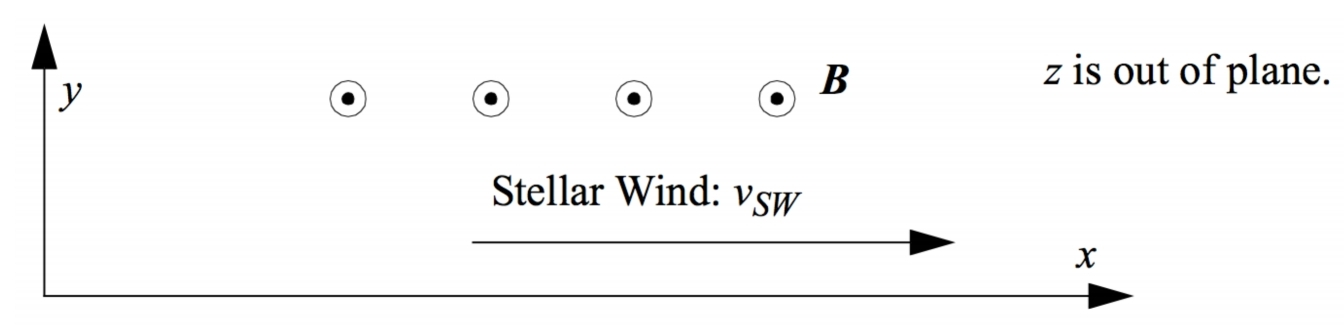
\includegraphics[width=0.7\textwidth]{hw2_p3.jpg} 
\end{center}

(1) Describe the subsequent motion of the $O^+$ ion, $x(t),y(t),v_x(t),v_y(t)$,
in our rest frame (not the plasma frame). \textit{Hint}: What is the solar wind
electric field? Calculate $v_x(t)$ and $v_y(t)$ then integrate. Apply boundary
conditions, $x(t=0)=0,y(t=0)=0,v_x(t=0)=0,v_y(t=0)=0$ to get an exact solution.

(2) Sketch the $O^+$ path.

(3) The drift and gyration cause the $O^+$ ion to slow down and speed up in our
rest frame. What is the drift speed? What is the gyration speed? What is the
maximum velocity (\si{km/s}) and energy (\si{keV}) that the $O^+$ ion reaches?

(4) Using the gyration speed only, what is the perpendicular (to $\vb{B}$)
temperature of that ion in $^\circ$\,\si{K}? (In 2D, temperature and energy are
equal.)
\begin{solution}
    (1) Assume an ideal plasma with $\vb{B}=B_0\zhat$ and
    $\vb{u}=v_{sw}\xhat$, then the electric field is
    \begin{equation}
        \vb{E}=-\vb{u}\times\vb{B}=v_{sw}B_0\yhat=E_0\yhat
    \end{equation}
    where $E_0=3.5$\,\si{mV/m}. Using the Lorentz force equation
    $\dot{\vb{v}}=(e/m)(\vb{E}+\vb{v}\times\vb{B})$ where $m$ is the mass of the
    $O^+$ ion, we get the following differential equations
    \begin{subequations}
        \begin{align}
            \dot{v_x}&=\frac{eB_0}{m}v_y=\Omega_cv_y\label{p3:vxd}\\
            \dot{v_y}&=-\Omega_c\qty(v_x-\frac{E_0}{B_0})\label{p3:vyd}
        \end{align} 
    \end{subequations}
    where $\Omega_c=eB_0/m$ is the unsigned cyclotron frequency. Taking another
    time derivative of \eqref{p3:vxd}, $\ddot{v_x}=\Omega_c\dot{v_y}$ and
    combining with \eqref{p3:vyd}, we can write an ODE in $v_x$
    \begin{equation}
        \ddot{v_x}=-\Omega_c^2\qty(v_x-\frac{E_0}{B_0}) 
    \end{equation}
    A general solution to this ODE is
    \begin{equation}
        v_x(t)=-v_\perp\cos\qty(\Omega_ct+\delta)+\frac{E_0}{B_0}
    \end{equation}
    It also follows from \eqref{p3:vxd} that
    \begin{equation}
        v_y(t)=-v_\perp\sin\qty(\Omega_ct+\delta) 
    \end{equation}
    At $t=0$, $v_y=0\Rightarrow\delta=0$. Then we can calculate
    $v_\perp=E_0/B_0=v_{sw}$ from requiring that $v_x=0$ at $t=0$. The solution 
    for the velocity is then
    \begin{subequations}\label{p3:velocity}
        \begin{align}
            v_x(t)&=-v_\perp\cos\qty(\Omega_ct)+\frac{E_0}{B_0}\\ 
            v_y(t)&=-v_\perp\sin\qty(\Omega_ct)
        \end{align} 
    \end{subequations}
    Integrating with respect to time, we get the position
    \begin{subequations}
        \begin{align}
            x(t)&=x_0+\frac{E_0}{B_0}t-\frac{v_\perp}{\Omega_c}\sin\qty(\Omega_ct)\\ 
            y(t)&=y_0+\frac{v_\perp}{\Omega_c}\cos\qty(\Omega_ct)
        \end{align} 
    \end{subequations}
    Setting $x(t=0)=0$ and $y(t=0)=0$, we find $x_0=0$ and
    $y_0=-v_\perp/\Omega_c$. The trajectory is then
    \begin{subequations}\label{p3:trajectory}
        \begin{align}
            x(t)&=\frac{E_0}{B_0}t-\frac{v_\perp}{\Omega_c}\sin\qty(\Omega_ct)\\ 
            y(t)&=\frac{v_\perp}{\Omega_c}\cos\qty(\Omega_ct)-\frac{v_\perp}{\Omega_c}
        \end{align} 
    \end{subequations}
    \eqref{p3:trajectory} and \eqref{p3:velocity} fully describe the subsequent
    motion of the ion.

    (2) See Figure~\ref{fig:p3}.
    \begin{figure}[h]
        \centering
        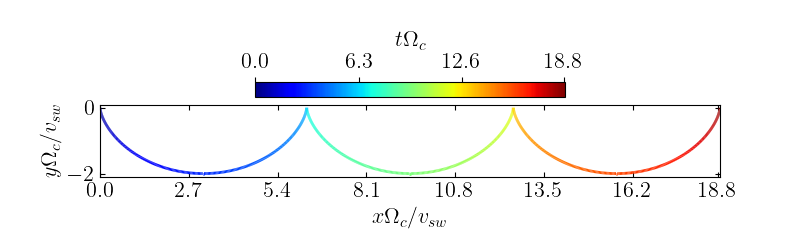
\includegraphics[width=0.8\textwidth]{p3.png}
        \caption{Trajectory of the $O^+$ ion, colored by time (from blue to
        red).}
        \label{fig:p3}
    \end{figure}

    (3) From \eqref{p3:velocity}, the drift speed ($E_0/B_0$) and the gyration 
    speed ($v_\perp$) are the same and they are both equal to
    $v_{sw}=350$\,\si{km/s}. From \eqref{p3:velocity}, the speed of the ion is
    \begin{equation}
        v=\sqrt{2(1-\cos(\Omega_ct))}v_\perp 
    \end{equation}
    This is maximum when $\Omega_ct=\pi$ ($v_y=0$; so the ion is at the turning 
    points in $y$), and $v_{\max}=2v_\perp=700$\,\si{km/s}. The rest mass of an
    oxygen ion is $m\approx14.92$\,\si{GeV}. Thus, the kinetic energy of this 
    ion travelling at $700$\,\si{km/s} is $E=(\gamma-1)m\approx40.7$\,\si{keV}
    where $\gamma$ is the Lorentz factor.

    (4) The perpendicular temperature is
    $T_\perp=(1/2)mv_\perp^2/k_B\approx1.2\times10^8$\,\si{K}.
\end{solution}
\end{problem}
%%%%%%%%%%%%%%%%%%%%%%%%%%%%%%%%%%%%%%%%%%%%%%%%%%%%%%%%%%%%%%%%%%%%%%%%%%%%%%%%
\begin{problem}{4}[Current sheet]
A current sheet is such that $\vb{J}$ is in the $y$ direction and $\vb{B}$ is in
the $z$ direction. $\vb{B},\vb{J}$, and $P$ vary only with $x$ (see diagram).
Derive a solution for $\vb{B}$, and $\vb{J}$ under the condition $\vb{J}\sim P$
that is valid for $-L<x<L$. Make sure that your solution satisfies the boundary
conditions of $\vb{B}(x=L)=-B_0\zhat$, and $\vb{B}(x=0)=\vb{0}$. $L$
is a characteristic length. Sketch your results.

\textit{Hint}: There is more than one possible solution -- just give any valid
solution. Be careful, the condition $\vb{J}^2\sim P$ is NOT the same as in the
Harris solution. 
\begin{solution}
    From the force equation, the total pressure is constant
    \begin{equation}
        \grad\qty(P+\frac{B^2}{2\mu_0})=0 
    \end{equation}
    Thus, the kinetic pressure is
    \begin{equation}\label{p4:P}
        P(x)=\frac{B_\infty^2-B^2(x)}{2\mu_0}
    \end{equation}
    where $B_\infty$ is the value of the magnetic field at the boundary and we
    have also set $P_\infty=0$. From Ampere's Law, $\partial B/\partial
    x=-\mu_0J_y=\mu_0A\sqrt{P}$ where $A$ is some constant such that
    $J_y^2=A^2P$. Combining this with \eqref{p4:P}, we can write
    \begin{equation}
        \frac{\partial B}{\partial
        x}=-A\sqrt{\frac{\mu_0}{2}}\sqrt{B_\infty^2-B^2(x)} 
    \end{equation}
    Since this is a separable differential equation, we can integrate for $B$
    \begin{equation}\label{p4:dB}
        -A\sqrt{\frac{\mu_0}{2}}\int dx=\int\frac{dB}{\sqrt{B_\infty^2-B^2}} 
    \end{equation}
    By a transformation $B=B_\infty\sin\theta$, \eqref{p4:dB}
    becomes
    \begin{equation}
        -A\sqrt{\frac{\mu_0}{2}}x=\int d\theta=\sin^{-1}\qty(\frac{B}{B_\infty}) 
    \end{equation}
    Inverting, we can write the magnetic field as
    \begin{equation}
        B(x)=-B_\infty\sin\qty(A\sqrt{\frac{\mu_0}{2}}x) 
    \end{equation}
    This immediately satisfies $B(0)=0$. However, we have to set
    \begin{equation}
        B_\infty=\frac{B_0}{\sin\qty(A\sqrt{\mu_0/2}L)} 
    \end{equation}
    So that $B(L)=-B_0$. The full solution for $\vb{B}$ is then
    \begin{equation}
        \vb{B}=-B_0\frac{\sin(A\sqrt{\mu_0/2}x)}{\sin\qty(A\sqrt{\mu_0/2}L)}\zhat
    \end{equation}
    The current is thus
    \begin{equation}
        \vb{J}=J_y\yhat=-\frac1{\mu_0}\frac{\partial B}{\partial x}\yhat 
        =-\frac{AB_0}{\sqrt{2\mu_0}}\frac{\cos\qty(A\sqrt{\mu_0/2}x)}{\sin\qty(A\sqrt{\mu_0}/2L)}\yhat
    \end{equation}
\end{solution}
\end{problem}
%%%%%%%%%%%%%%%%%%%%%%%%%%%%%%%%%%%%%%%%%%%%%%%%%%%%%%%%%%%%%%%%%%%%%%%%%%%%%%%%
\begin{problem}{5}[Magnetic diffusion]
Consider a magnetic field $\vb{B}=B_z(x,t)\zhat$ where
$B_z(x,t=0)=B_0\cos(k_1x)+B_0\cos(k_2x)$ in a resistive plasma with $k_2\gg
k_1$.

(a) Find the solution for $B_z(x,t)$.

(b) Sketch (accurate plot not needed) the solution for $t=0$ and $t>0$. What
happens to the high-$k$ wave?
\begin{solution}

    (a)
    The 1D diffusion equation is
    \begin{equation}\label{p5:deq}
        \frac{\partial B_z}{\partial
        t}=\frac1{\sigma\mu_0}\frac{\partial^2B_z}{\partial x^2} 
    \end{equation}
    where $\sigma$ is the electric conductivity of the plasma such that
    \begin{equation}
        \vb{E}+\vb{u}\times\vb{B}=\frac{\vb{J}}{\sigma} 
    \end{equation}
    The differential equation \eqref{p5:deq} can be solved by separation of
    variables. Let us write $B_z(x,t)=X(x)T(t)$ and plug it back into
    \eqref{p5:deq}
    \begin{equation}
        \frac{T'(t)}{T(t)}=\frac1{\sigma\mu_0}\frac{X''(x)}{X(x)}
    \end{equation}
    The LHS is completely dependent on time, while the RHS is dependent on the
    position $x$. Thus, they must equate to a constant $-\gamma$. We then have
    the following two ordinary differential equations
    \begin{subequations}
        \begin{align}
            \frac{dT}{dt}&=-\gamma T(t) \label{p5:dT}\\
            \frac{d^2X(x)}{dx^2}&=-\gamma\sigma\mu_0X(x)\label{p5:dX}
        \end{align} 
    \end{subequations}
    The general solution to \eqref{p5:dT} is $T(t)=e^{-\gamma t}$, while the
    general solution to \eqref{p5:dX} is
    \begin{equation}
        X(x)=a\sin(kx)+b\cos(kx) 
    \end{equation}
    such that
    \begin{equation}\label{p5:kgamma}
        k^2=\gamma\sigma\mu_0 
    \end{equation}
    However, note that at $t=0$, $B(x,0)$ is an even function in $x$. Thus, 
    there cannot be any sine dependence and $a$ must be zero. Then the magnetic 
    field can be written as a linear combination of these orthogonal functions
    \begin{equation}
        B_z(x,t)=\sum_{n\in\N}b_ne^{-\gamma_nt}\cos(k_nx)
    \end{equation}
    where $\gamma_n,k_n$ follow the relation in \eqref{p5:kgamma}. At $t=0$, we
    have
    \begin{equation}
        B_z(x,0)=B_0\cos(k_1x)+B_0\cos(k_2x)=\sum_{n\in\N}b_n\cos(k_nx) 
    \end{equation}
    By symmetry, we must require that $b_n=0$ where $n\neq1$ or 2 and that
    $b_{1,2}=B_0$. The solution for the magnetic field is then
    \begin{equation}\label{p5:B}
        B_z(x,t)=B_0e^{-k_1^2t/\sigma\mu_0}\cos(k_1x)+B_0e^{-k_2^2t/\sigma\mu_0}\cos(k_2x) 
    \end{equation}

    (b) Let the normalized position be $\overline{x}=k_2x$ and normalized time
    be $\overline{t}=k_2^2t/\sigma\mu_0$. Also, let $\epsilon=k_1/k_2\ll1$. Then
    from \eqref{p5:B}, the normalized magnetic field $\overline{B}=B_z/B_0$ is
    \begin{equation}
        \overline{B}=e^{-\epsilon^2\overline{t}}\cos(\epsilon\overline{x})+e^{-\overline{t}}\cos(\overline{x}) 
    \end{equation}
    In this form, it is clear that the decay rate in the low $k$ wave (first
    term) is much smaller than that in the high $k$ wave (second term). Thus, 
    we expect the high $k$ wave to damp away much sooner than the low $k$ wave. 
    This is demonstrated in Figure~\ref{fig:p5} where we have plotted the 
    magnetic field $\overline{B}$ with $\epsilon=0.1$.
    \begin{figure}[h]
        \centering
        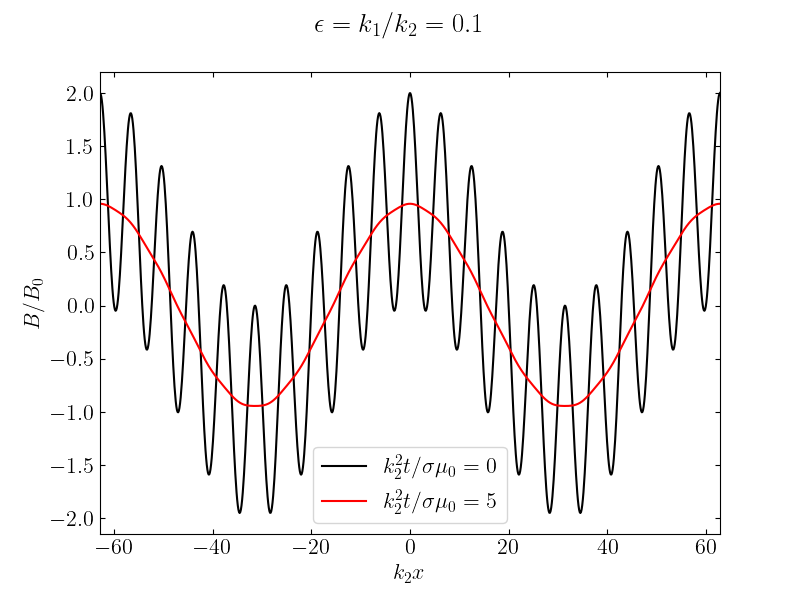
\includegraphics[width=0.7\textwidth]{p5.png}
        \caption{Magnetic field solution in spatial domain at
        $\overline{t}=0$ (black) and $\overline{t}=5$ (red).}
        \label{fig:p5}
    \end{figure}
\end{solution}
\end{problem}
%%%%%%%%%%%%%%%%%%%%%%%%%%%%%%%%%%%%%%%%%%%%%%%%%%%%%%%%%%%%%%%%%%%%%%%%%%%%%%%%

\end{document}
